%%%%%%%%%%%%%%%%%%%%%%%%%%%%%%%%%%%%%%%%%%%%%%%%%%%%%%%%%%%%%%%%%%%%%%%%%%%%%%%%
% Diese Datei beinhaltet den eigentlichen Inhalt Ihrer Arbeit.
%
% Es bietet sich der Übersicht halber an, die einzelnen Abschnitte jeweils
% in eigene Dateien zu schreiben und mittels \input einzubinden.
% Eine mögliche Verzeichnisstruktur sähe entsprechend so aus:
%
%     thesis/
%     +- tex/
%     |  +- introduction.tex
%     |  +- motivation.tex
%     |  +- experiments.tex
%     |  |  ...
%     |  +- conclusion.tex
%     +- abstract.tex
%     +- contents.tex
%     +- thesis.tex
%%%%%%%%%%%%%%%%%%%%%%%%%%%%%%%%%%%%%%%%%%%%%%%%%%%%%%%%%%%%%%%%%%%%%%%%%%%%%%%%

\section{Introduction}

For this thesis a Java library called \verb|gp-modifiable-ast| was implemented. 
\verb|gp| stands for general purpose, meaning that it can provide the API for different grammars, for example for different programming languages.

\subsection{Motivation}

The motivation for this work came from a practical problem. 
While developing a large enterprise web application, there was a need to change the translation system.
A translation system is receiving a token as a string and returns a predefined translation depending on the target language.
This caused some issues, as the new translation system had a different call syntax as the old one.
This refactoring required looking into external data stored in a database for each different call the translation function.
Because of the dependency of external data, the automatic tools provided by the IDE have not been sufficient to refactor these calls.

On the other hand, this would have been a very time consuming task to perform manually, as over tenthousand calls to this function existed.

To resolve this issue, a specific JavaScript parser like Esprima \cite{esprima} was used. 
Esprima can parse JavaScript, provide an AST, allows modifications on the AST and conversion back to source code.
With this library it was possible to perform the refactoring with the necessary customization options and accuracy.

However, tools like Esprima mostly exist for well known programming languages, and each tool provides a different API.

While there are parser generators like SableCC \cite{sablecc}, which can generate parsers from a definition file, they are intended to be used for a different
purpose.
Common parser generators are implemented to provide a part of a compiler frontend, but they do not need to maintain whitespaces,
comments and be able to generate the original source code from the ast.

The goal of this work is to provide a library called \verb|gp-modifiable-ast| to minimize the effort needed to be able to perform manipulations directly on the AST and
beeing able to transform the AST back into source code with the least amount of changes needed.

The following example should illustrate that rewritable abstract syntax trees can be used for refactorings, which require some knowledge about the program structure.
The change that should be performed on the following source code is renaming all variables to enforce a camel case naming scheme on variables, while keeping
pascal case on function names. While this can be done with IDE tools, it would require manual effort every time.

Implementing a custom solution can enforce this naming scheme automatically.

\begin{lstlisting}[language=Java, caption=Example of untransformed code]
void should_be_snake_case(int should_be_camel_case) {
    int second_variable = should_be_camel_case;
}
\end{lstlisting}

The resulting AST from this code may look like this
\begin{figure}[H]
    \centering
    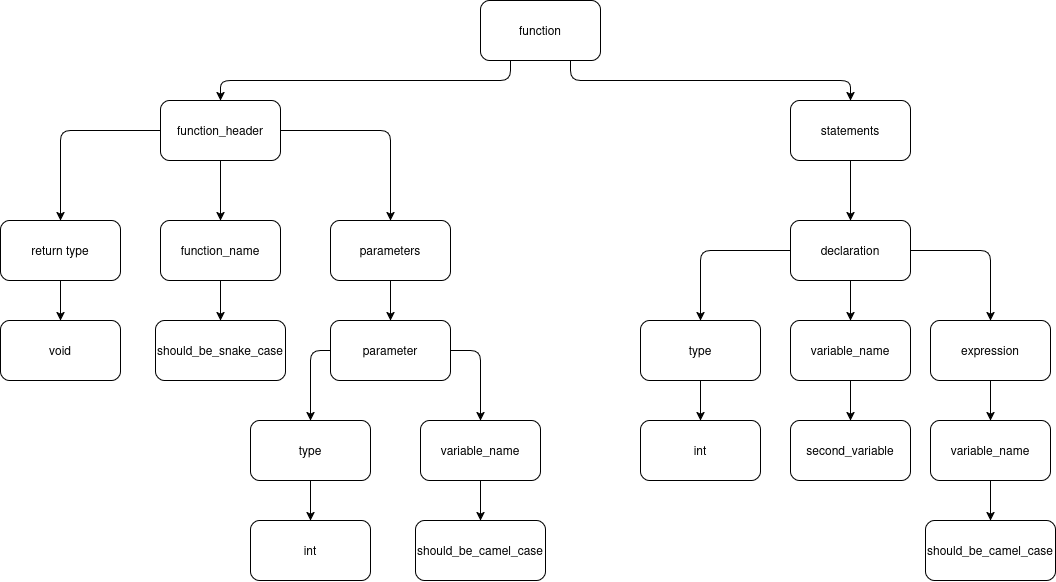
\includegraphics[scale=0.40]{fig/ast_example.png}
    \caption{AST example}
\end{figure}

This AST contains alot of informations about the program structure and allows to differentiate between variable and function names
\footnote{
    Depending on the grammar and language, this differentiation may not always be possible on the generated AST. 
    For example in JavaScript, functions can be passed as parameters into other functions: 
    \lstinline{function\_a(function\_b, variable\_a)}.
    The implemented LR(1) parser is not able to differentiate between the types of the parameters in this case.}. 

The following code should represent the general idea on how transformations on the AST could be implemented. 
The API of \verb|gp-modifiable-ast| is different from this example.

\begin{lstlisting}[language=Java, caption=Example of transformation]
    AST ast = parser.parse("example.java");
    List<ASTNode> nodes = ast.find("variable_name");
    renameToCamelCase(nodes);
    ast.transformBackToSourceCode();
\end{lstlisting}

This transformation would result in the following code.

\begin{lstlisting}[language=Java, caption=Example of transformation]
void should_be_snake_case(int shouldBeCamelCase) {
    int secondParam = firstParam;
}
\end{lstlisting}

This example should illustrate why rewritable abstract syntax trees can be a usefull tool for software development, as they allow a vast range of refactorings by containing
informations about the program structure.

\subsection{Related work}

The library implemented for this thesis (\verb|gp-modifiable-ast|) has similarities to common parser generators like SableCC \cite{sablecc}, ANTLR \cite{antlr}, GNU Bison \cite{gnu-bison} and others.

There are custom parsers like Esprima \cite{esprima}, which can generate a modifiable AST for JavaScript sources, but those are limited to one specific programming
language.

\verb|gp-modifiable-ast| is able to maintain the original formatting as much as possible and can be defined for any grammar that can be parsed by an LR(1) parser.

This work is based on the conference paper of Jeffrey L. Overbey and Ralph E. Johnson with the title "Generating Rewritable Abstract Syntax Trees" \cite{GeneratingRewritableAST}.
In this paper a possible grammar definition for rewritable abstract syntax trees is defined, which \verb|gp-modifiable-ast| implements partially. 
Some of the proposed definitions of \cite{GeneratingRewritableAST} have not been implemented, as those would not serve any purpose with the
structure of \verb|gp-modifiable-ast|. In chapter \ref{chap:ast_generation} it is discussed, which ones are implemented and which ones are not.

\section{Prerequisites}

In this chapter we want to establish the prerequisites required to understanding this thesis.

\subsection{Regular Expressions and Grammars}

In theoretical computer science, a grammar consists out of a set $\Sigma$ of terminal symbols, a set $N$ of nonterminal symbols, a set $P$ of productions and a start symbol $S$. $S$ is always a nonterminal symbol and therefore $S \in N$. The productions are defined as $P \subseteq (N \cup \Sigma)^+ \times (N \cup \Sigma)^*$. The $^+$ refers to one or more, the $^*$ refers to zero or more.

Grammars can be seperated in different different classes based on the chromsky hierarchy. The main ones we are looking at in this thesis are the contextfree grammars and the regular grammars.

A grammar is context free, if for all productions $p \to q$ in $P$ the following applies: $p \in N$.

A grammar is a regular grammar, if for all produtions $p \to q$ in $p$ the following applies: $p \in N$ and $q \in \Sigma \cup \Sigma N$.

Grammars are used, because they can describe a language. In our use case, they describe an programming language and can be used, to parse the source code. Regular expressions are short statements, that avoid defining an entire grammar definition. Their downside is, that they are not able to describe alot of the features modern programming languages have. For example, it is not possible to write a regular grammar for the language that has the same amount of opening and closing brackets. An example for a regular expression would be this:

\begin{align*}
a^*ba^*b
\end{align*}

This would parse all words that have any amount of "a", followed by exactly one b, followed by any amount of "a", followed by exactly one b.

To handle these situations, we require the context free grammars, they are able to parse more cases and are sufficient enough, to parse most programming languages. However, even the context free grammars are not powerfull enough to correctly verify if a given source code is valid. For this, we would technically need context sensitive grammars. Those come with the cost of a worse runtime, therefore usually context free grammars are used when writing compilers and additional verifications are done after the parsing to ensure the language is indeed valid source code.

An example for a context free grammar:

Let $\Sigma = \{E\}, N = \{a, b\}, S = \{E\}$ and the productions defined as:

\begin{align*}
P = \{&E \to a E b,\\
&E \to \epsilon\}
\end{align*}

$\epsilon$ is a special symbol, it refers to the empty word. That means, that $E$ can be derived to nothing. Without this, we would have endless self recursion in the grammar rule.

This grammar would be equivalent to the opening and closing bracket example from previously. This will parse any string, which has for one opening a exactly one opening b.


\subsection{Lexer}

The parse process of a compiler is often times split into two parts. The first part is the so called lexer. The task of the lexer is to take in the entire source code and create a so called token stream. The lexer usually can mostly run with regular expressions and avoids context free grammars for the most part.

The lexer is a preparation for the parser, as it removes unwanted characters like whitespaces and generalizes other tokens by already classifying them for their intended use case. For example could be any string matching the regular expression \verb|[a-zA-Z_][a-zA-Z_0-9]*| an identifier and \verb|[0-9]+| would be an integer. The name identifier is often used for variable, function and classnames in lexers. By doing this, the parser later only needs to work with the abstract identifier, not with the real input.

\subsection{Parser}

The second part will perform the parsing on the token stream and by using the grammar rules. There are many kinds of parsers, the most common ones used in compiler development are:

\begin{enumerate}
\item LL(1): Scanning the input from left to right, applying leftmost deriviation, using one token of lookahead.
\item LR(1): Scanning the input from left to right, applying rightmost deriviation, using one token of lookahead.
\item LALR(1): A variation of LR(1), which reduces the amount of calculations and memory requirements.
\end{enumerate}

There are two goals of the parsing process. The first one is to verify that the input matches the grammar. The second one is to generate a tree structure, which represents the input. The tree structure generated by the parser is called a concrete syntax tree (CST). This tree structure is very verbose and represents the grammar definition exactly.

There are two main different ways used to parse source code. The first approach is top-down parsing. In top-down parsing, the root node will be generated first, following by the childrens and the leaf nodes will be generated at the end. LL(1) parsing is one example for top-down parsing. The other approach is bottom-down parsing. In this parsing strategy the leaf nodes are generated first and the root node is generated at the very end. LR(1) and LALR(1) are examples for bottom-down parsing algorithms.

The top-down parsers have the benefit of being rather easy to understand, however they are less powerfull. Bottom-down parsers are harder to understand and to debug, however they can parse more grammars.

Each of the presented grammars are not able to parse all context free grammars, but they are sufficient enough to parse most programming languages. LR(1) is the parsing strategy that is able to parse the most grammars, but requires the largest amount of memory and calculations to correctly parse.

As memory and runtime is not the main priority in this thesis, a LR(1) parser was implemented to allow the largest amount of grammars being parsed.

\subsubsection{LR(1)-Parsing}

The LR(1) parsing strategy relies on two different tables. The first table is called an action table. The rows represents different states. The columns represent the terminal symbols of the grammar. The value of each cell can be empty, a shift, a reduce or an accept action. 

A shift action will consume a token from the token stream and move to a new state.

A reduce action will go back to a previously encountered state and references a grammar rule that is beeing reduced.

A accept action is only defined once in the entire table. Once this is encountered, the parsing process is finished and the input was successfully parsed.

The second table is the goto table. The rows represents the different states. The columns represent the non terminal symbols of the grammar. The content of each cell can either be a reference another state or empty.

The parser itself manages a stack of states. The top of the stack is the current state that is currently being processed. The parser reads the current token in the token stream provided by the lexer and receives the current action from the action table.
Based on the action type, different behaviours apply.

On a shift action, the parser will shift the position in the token stream and will continue in the next iteration with a new token. The new state defined in the shift action will be pushed on the stack. Then the next iteration is started.

On a reduce action, the parser will pop as $n$ states from the stack, where $n$ is equal to the amount of terminal and nonterminal symbols on the right hand side of the grammar rule. Afterwards, the new top of stack is beeing read and the state defined in the goto table of the top of stack and the current token in the token stream will be pushed on the stack.

On an accept action, the parser will finalize the parsing process accept the input. 


\subsubsection{Preprocessor Statements}

Hier kurz darauf eingehen, was preprocessor statements sind.

\section{Implementation}

\subsection{Class generation vs general classes}

Mostly, parser generators will create classes for every production. This allows the user to modify the generated classes, for example adding new methods. This allows for better usablility if done correctly. We chose to not follow this approach, instead we have a small set of predefined classes, which are used across all nodes. With this approach, no additional code generation for the parser is needed. The parser can run standalone and in place. This approach allows for an easier introduction to the system, as a grammar and a source file can simply be passed to the parser generator and an AST will be generated. Otherwise, first the parser needs to be generated and afterwards the parser needs to be called to parse the source files.

\subsection{Extendability}

Hier darauf eingehen, in wie weit das Programm erweiterbar ist. Welche Möglichkeiten existieren in den Lexer/Parser einzugreifen?

\subsection{Grammar file syntax}

The productions and lexer definitions are defined seperately from the implementations in their own text files. Each language has exactly one text file defining the productions and lexer definitions. The contents are seperated in four different chapters.

The first chapter is \verb|LANGUAGE_DEF|. This contains various general definitions for the language. This chapter contains e.g. what comment styles are allowed and how they are identified, name of the language, file extension used, wether or not the language is case sensitive and what production should be used as the starting production. All settings here are defined as key, value pairs.

The second chapter is the \verb|LEXER_RULES|. In there, we define all tokens that can appear in the source file and that the lexer should handle. The lexer can handle three different types of definitions. The first type is matching a fixed string. The second type matches a regex. The last type uses a custom implementation to check for a match. The last matching matching definition wins. For example, the token definition \verb|true_literal = "true";| and the definition \verb|identifier = regex([a-zA-Z_][a-zA-Z_0-9]*);| would both match the string \verb|true|. Therefore, the more general \verb|identifier| token should be defined before the \verb|true_literal| token. This will cause the lexer to identify the text \verb|true| as \verb|true_literal|. A lexer key needs to be written in all lowercase (and lowercase) letters.

The chapter \verb|HIDDEN_LEXER_RULES| is a comma seperated list of lexer definitions keys, which should not be handled in the parse process and also not be visible in the AST by default. 

The chapter \verb|GRAMMAR_RULES| contains all productions of this language. The syntax is similar, but not equal, to the backus natus form. (TODO: Source). The syntax was extended by most of the modifiers proposed by \cite{GeneratingRewritableAST}. The terminals are the keys of the lexer definitions. The nonterminals are defined by the left hand sides of the productions. All nonterminals have to be written in uppercase and underscores. \verb|EPSILON| is used for the empty word. Every terminal and nonterminal symbol can be extended by a list of modifiers in square brackets after the name. \verb|FORMAL_PARAMETER -> TYPE identifier[alias=parameterName];| defines the production with \verb|FORMAL_PARAMTER| on the left hand side and \verb|TYPE identifier| on the right hand side. \verb|TYPE| references a different production. \verb|identifier| references a lexer definition. \verb|[alias=paramterName]| sets the alias modifier onto the \verb|identifier| symbol.

\subsection{CST-Generation}

The concrete syntax tree (CST) is a tree structure, that matches the the grammar and lexer definitions exactly. Our CST also should contain nodes, which are usually omitted, like comments or whitespaces.

The CST is implemented by a \verb|ConcreteSyntaxTreeNode| class. A node can either reference a production or a lexer token. We maintain the production, as these allow us to perform advanced modifications and generate a less verbose abstract syntax tree from the cst. The lexer tokens are maintaned, as these include the original sources.

This structure is generated by the parser directly. The parser manages a second stack, containing tree nodes that are not attached to a parent node.

As the parser is progressing through the token stream provided by the lexer, it generates new tree nodes and pushes them on the stack whenever either the token is contained in \verb|HIDDEN_LEXER_RULES| or the action performed is a shift action. 

On a reduce action, the parser will also create a new tree node. This tree nodes will have other tree nodes from the top of the stack as children. This behaviour is very similar to the behaviour how the state stack of the parser manages its state. The main difference are the tokens in the \verb|HIDDEN_LEXER_RULES|. The reduced production might only have one symbol on the right hand side, but on the tree node stack are two nodes from \verb|HIDDEN_LEXER_RULES|. In this case, the parser will pop three states from the top of the tree node stack and add them as children of the newly created node in reverse order. In case the parser reaches the \verb|acc| state, it will not be guaranteed that the stack only contains the root node though. There might be tokens from \verb|HIDDEN_LEXER_RULES|, which appeared at the start of the parsed string. Therefore, the parser will find the root node, and prepend all remaining entries in the tree node stack to the childrens of the root node. 

With this algorithm, every single token from the token list of the lexer will be transformed into a tree node and will be in the CST. This guarantees, that the entire source code is represented in the CST and the CST could be transformed back to the source code exactly.

\subsection{AST-Generation}

The AST consists of three different node types. \verb|ProductionTreeNode| are nodes that originated from a grammar production. \verb|TokenTreeNode| are nodes that originated from a lexer token. \verb|StringTreeNode| are nodes that contain a string and are used to replace other tree ndoes. These nodes are usually not part of the initial AST, they can be added later on to the AST.

The AST is created from the CST. The \verb|TokenTreeNode| which reference a token from \verb|HIDDEN_LEXER_RULES| will marked as hidden. These nodes are stored in the AST, but they will not be visible to the user, unless specifically requested. Afterwards, the AST structure will be modified by the modifiers defined in the grammar file. Each modifier has their own implementation and will be applied bottom up for each node.

\subsubsection{list-Modifier}

The \verb|list| modifier, purposed by \cite{GeneratingRewritableAST}, is a modifier that is supposed to flatten out self recursive productions. This modifier can only be applied to symbols on the left hand side of a production. The following example might be a production for the function paramters in common programming languages.

\begin{verbatim}
FORMAL_PARAMETER_LIST[list] -> FORMAL_PARAMETER_LIST FORMAL_PARAMETER | FORMAL_PARAMETER | EPSILON;
\end{verbatim}

Without the \verb|[list]| modifier, this would create a tree structure like this

\newpage

\begin{enumerate}
\item	\verb|FORMAL_PARAMETER_LIST|
\begin{enumerate}
\item	\verb|FORMAL_PARAMETER_LIST|
\begin{enumerate}
\item \verb|FORMAL_PARAMETER|
\end{enumerate}
\item \verb|FORMAL_PARAMETER|
\end{enumerate}
\item \verb|FORMAL_PARAMETER|
\end{enumerate}

Mostly, we do not want a structure like this. By applying the \verb|list| modifier, the resulting structure will be:

\begin{enumerate}
\item	\verb|FORMAL_PARAMETER_LIST|
\begin{enumerate}
\item \verb|FORMAL_PARAMETER|
\item \verb|FORMAL_PARAMETER|
\item \verb|FORMAL_PARAMETER|
\end{enumerate}
\end{enumerate}

This structure is much easier to manage and still contains all relevant informations about the sources.

The modifier is applied by checking if the children of the current \verb|ProductionTreeNode| $n$ contains a \verb|ProductionTreeNode| $m$ referencing the same production. If this is the case, $m$ is replaced in the children list of $n$ by all childrens of $m$.

\subsubsection{alias-Modifier}

The \verb|alias| modifier, purposed by \cite{GeneratingRewritableAST}, is a modifier that can be applied to any symbol in the right hand side of a production. This modifier, will add an alias to the tree node, which can be used to search the tree. The following might be an example for a production for addition in a programming language.

\begin{verbatim}
ADD -> NUMBER[alias=left] plus NUMBER[alias=right];
\end{verbatim}

Without the alias modifier, the only way to differentiate between the both \verb|NUMBER| nodes would be by the order of the children of the \verb|ADD| tree node. The \verb|alias| modifier allows for cleaner searches in the AST.

This modifier is applied by simply storing the alias in the tree node.


\subsubsection{hidden-Modifier}

The \verb|hidden| modifier, purposed by \cite{GeneratingRewritableAST}, is a modifier that can be applied to terminal symbols in the right hand side of a production. This modifier will hide the tree node in the AST. In the previous example of the \verb|ADD| production, the \verb|ADD| tree node would have a \verb|TokenTreeNode| child, which references the \verb|plus| lexer definition. This information is obsolute, as the production will always contain this node and the production name already contains the necessary informations. By applying the \verb|hidden| modifier to the \verb|plus| symbol, the corresponding tree node will still be present, but not visible unless specifically requested.

\subsubsection{inline-Modifier}

The \verb|inline| modifier, purposed by \cite{GeneratingRewritableAST}, is a modifier that can be applied to nonterminal symbols in the right hand side of a production. 

By applying the modifier, the node will be replaced with all its children. This modifier should be used on nonterminals, which itself do not carry important informations, but their children do. This way all informations are maintaned, but the tree structure gets simplyfied.

\subsubsection{Not implemented modifiers}

\cite{GeneratingRewritableAST} purposed additional modifiers, those are not implemented currently. That would be the \verb|Boolean Access| modifier, which would replace a node with a boolean value. However, as we do not generate classes for each production, this would serve little purpose for us. The same reason applies to the \verb|superclass| modifier, which would create a hierarchy in the generated classes of the parser generator.

\subsection{AST search methods}

Before any modification can be applied to the AST, firstly the nodes have to be found which can be modified.

For this approach, each ast node has three methods.

\begin{enumerate}
\item \verb|query: Selector -> QueryResult|
\item \verb|queryChildren: Selector -> QueryResult|
\item \verb|queryImmediateChildren: Selector -> QueryResult|
\end{enumerate}

The \verb|query| methods takes a selector and returns a \verb|QueryResult|. The \verb|QueryResult| contains all nodes in the subtree of the searched node which match the \verb|selector|. The \verb|QueryResult| can also contain the searched node itself.

The \verb|queryChildren| behaves the same, but will not include the searched node itself.

The \verb|queryImmediateChildren| will only include the immediate children of the searched node matching the \verb|selector|.

The \verb|QueryResult| instance also allows to perform queries on the result. This will perform the according method on all nodes in the result and create a new \verb|QueryResult| instance containing the merged results of each node. This allows for easy chaining of selectors. Also \verb|QueryResult| instances can be merged for further processing with the \verb|merge| function.

\subsection{Selectors}

A \verb|Selector| is a classinstance, which should test wether a given treenode matches the rules defined by the \verb|Selector|. The \verb|Selectors| can be splitted into three different categories.

The first category are logical \verb|Selectors|. They should represent logical operations. There are two \verb|Selectors| defined by default, \verb|AndSelector| and \verb|OrSelector|. Each of them takes a list of other selectors. The \verb|AndSelector| will only match tree nodes, that match all passed \verb|Selectors|. The \verb|OrSelector| will match all tree nodes, where atleast one of the passed \verb|Selectors| match the node.


The second category are data \verb|Selectors|. Those selectors search for nodes based on the data contained in them. These can match the name of a production, the alias of a production, the name of a lexer definition and the value of a lexer token. The implemented selectors are \verb|AliasSelector|,\verb|ProductionSelector|,\verb|TokenSelector|,\verb|TokenValueSelector|. All of those receive a string as a parameter and check the corresponding notes for this string.


The last category are structural \verb|Selectors|. Those selectors search for nodes that have specific nodes in the children or parents. 

The following example of an AST should show the purpose of this category.
\begin{enumerate}
\item \verb|METHOD_CALL|
\begin{enumerate}
\item \verb|CALLED_ON|
\begin{enumerate}
\item \verb|translator|
\end{enumerate}
\item \verb|METHOD_NAME|
\begin{enumerate}
\item \verb|translate|
\end{enumerate}
\end{enumerate}
\end{enumerate}
To search for all \verb|METHOD_CALL| nodes, that call translate on a translator object, we will want these types of selectors.

An example selector for this would be

\begin{verbatim}
new AndSelector(
	new ProductionSelector("METHOD_CALL"),
	new HasImmediateChildSelector(
		new AndSelector(
			new ProductionSelector("CALLED_ON"),
			new HasImmediateChildSelector(
				new TokenValueSelector("translator")
			)
		)
	),
	new HasImmediateChildSelector(
		new AndSelector(
			new ProductionSelector("METHOD_NAME"),
			new HasImmediateChildSelector(
				new TokenValueSelector("translate")
			)
		)
	)
)
\end{verbatim}

By calling the \verb|query| method on the root node of the AST, we will receive all \verb|METHOD_CALL| nodes in the AST matching these conditions.

\subsection{AST Modifications}

The \verb|AbstractSyntaxTreeNode| class contains multiple methods to make modifications.

\begin{enumerate}
\item \verb|replace|  Replaces this node with a list of other nodes.
\item \verb|replaceChild|  Replaces a node in the childrens with a list of other nodes.
\item \verb|remove| Removes this node
\item \verb|removeChild| Removes a child
\item \verb|addChild| Adds a child to the end of the children list
\item \verb|addChildBefore| Adds a child before another node.
\item \verb|addChildAfter| Adds a child after another node.
\item \verb|deepClone| Clones this node and all childrens, returns a node that equals the current one but without a parent reference.
\end{enumerate}

Each \verb|AbstractSyntaxTreeNode| references their corresponding parent node. To maintain integrity, you can only add nodes that have no parent node and replace only nodes with a parent reference. To add a node to multiple other nodes, you can clone the node to be added.

\subsection{Extendability}

To allow for the largest amount of possible extendability, we allow for various ways of customization

\subsubsection{Lexer}

As mentioned before, the lexer definitions can contain custom matchers. Those matchers are custom implementations, which are referenced by a name in the grammar file. These classes are written by the user and registered by calling \verb|CustomMatcherRegistry.registerCustomMatcher|. A custom matcher needs to implement the \verb|ICustomMatcher| interface. A matcher gets a \verb|LexerContext| and returns \verb|null| or the matched string. By the \verb|LexerContext| parameter, the matcher can receive the remaining input and checks if the beginning of the remaining input can be tokenized by this matcher.

\subsubsection{Parser}

???


\subsubsection{AST Generation}

We allow for various ways for custimizing the AST generation. Firstly, custom modifiers for grammar symbols can be implemented. Also, the AST can be postprocessed and decorated. For example, the tree ndoes can be replaced with their own implementation, they simply need to extend \verb|AbstractSyntaxTreeNode|.

\subsubsection{Selectors}

Custom selectors can be defined by implementing \verb|ISelector|. Those can simply be defined and used with the query methods of the tree node.

\section{Proof of concept}

\subsection{Java Subset}

Hier kurz darauf eingehen, für welche Sprache eine Grammatik definiert wurde.

\subsection{Automated Refactoring}

Hier Beispiel/Beispiele für automatisierte Refactorings anführen. Beispielsweise Funktionsnamen von underscore zu camelCase überführen.

\section{Conclusion}

Am Ende der Arbeit werden noch einmal die erreichten Ergebnisse
zusammengefasst und diskutiert.
